\documentclass[../../../doc/main]{subfiles}
\begin{document}
    \setcounter{chapter}{1}
    \setcounter{section}{2}
    \section{解説}\label{解説1}
        \begin{enumerate}
            \item [\kakkoichi]
            \textcolor{myBlue2}{$A_k$に関して,被積分関数が絶対値の形となっています.積分の計算をするためには絶対値を外す必要がありますが,
            本問では不等式評価をするのみであるので,一旦は置いておきます.絶対値の中に注目してみましょう.$\sin{(x^2)}$は
            $f(x)=\sin{x},~g(x)=x^2$としたときの合成関数$f(g(x))$になっています.被積分関数が合成関数になっているとき,
            $t=g(x)$と置換するとうまくいくことが多いです(経験則です).}\\
            $t=x^2$と置換する.積分区間を考えると$x>0$であることから,$x=\sqrt{t}$であることが分かる.
            \begin{align*}
                \yueni~~A_k=\dint{k\pi}{(k+1)\pi}\emabs{\sin{t}}\sdot\bunsuu{dt}{2\sqrt{t}}
                \quad\quad\quad\quad\quad
                \begin{tabular}{|c|c|} \hline
                    $x$ & $\sqrt{k\pi}\to\sqrt{(k+1)\pi}$\bsityuu \\ \hline
                    $t$ & $k\pi\to(k+1)\pi$\bsityuu \\ \hline
                \end{tabular}
                \quad\quad \bunsuu{dt}{dx}=\bunsuu{1}{2\sqrt{t}}
            \end{align*}
            \textcolor{myBlue2}{ほら!積分区間,被積分関数の両方とも見た目がスッキリしたでしょう?次に考えるべきは,積分の不等式評価です.
            積分区間は$k\pi\leq t\leq(k+1)\pi$となっています.これより$t$の最大値が$(k+1)\pi$で最小値が$k\pi$であることが分かります.したがって,
            $0<k\pi\leq t\leq(k+1)\pi$より}
            \begin{align*}
                \textcolor{myBlue2}{\bunsuu{1}{(k+1)\pi}\leq \bunsuu{1}{t}\leq \bunsuu{1}{k\pi}\Y \bunsuu{1}{\sqrt{(k+1)\pi}}\leq \bunsuu{1}{\sqrt{t}}\leq \bunsuu{1}{\sqrt{k\pi}}~\sdots\sdots~\maruichi}
            \end{align*}
            \textcolor{myBlue2}{が得られます.示すべき不等式の形が見えてきました!}\\
            ゆえに\textcolor{myBlue2}{($\maruichi$と$\emabs{\sin{t}}\geq 0$より)}
            \begin{align*}
                &\dint{k\pi}{(k+1)\pi}\emabs{\sin{t}}\sdot\bunsuu{dt}{2\sqrt{(k+1)\pi}}\leq \dint{k\pi}{(k+1)\pi}\emabs{\sin{t}}\sdot\bunsuu{dt}{2\sqrt{t}} \leq \dint{k\pi}{(k+1)\pi}\emabs{\sin{t}}\sdot\bunsuu{dt}{2\sqrt{k\pi}}\\
                &\yueni~~\dint{k\pi}{(k+1)\pi}\emabs{\sin{t}}\sdot\bunsuu{dt}{2\sqrt{(k+1)\pi}}\leq A_k \leq \dint{k\pi}{(k+1)\pi}\emabs{\sin{t}}\sdot\bunsuu{dt}{2\sqrt{k\pi}} \\
                &\yueni~~\bunsuu{1}{2\sqrt{(k+1)\pi}}\dint{k\pi}{(k+1)\pi}\emabs{\sin{t}}\,dt\leq A_k \leq \bunsuu{1}{2\sqrt{k\pi}}\dint{k\pi}{(k+1)\pi}\emabs{\sin{t}}\,dt
            \end{align*}
            \textcolor{myBlue2}{被積分関数$\bunsuu{\emabs{\sin{t}}}{2\sqrt{t}}$のうち,分子の$\sqrt{t}$の部分のみ不等式で評価をしました.分母の$\emabs{\sin{t}}$も同様にやったらどうでしょう?
            より式が複雑になってしまいそうです.ここまで来たら,$\dint{k\pi}{(k+1)\pi}\emabs{\sin{t}}\,dt=2$となることが示されれば証明完了ですね.周期性から,$\dint{k\pi}{(k+1)\pi}\emabs{\sin{t}}\,dt$の値は$y=\emabs{\sin{t}}$
            のお山1つ分(下図の斜線部)の面積と等しくなります.(お山1つ分の面積が2になることは覚えておきましょう!)}

            \begin{figure}[htbp]
                \centering
                \textcolor{myBlue2}{
                    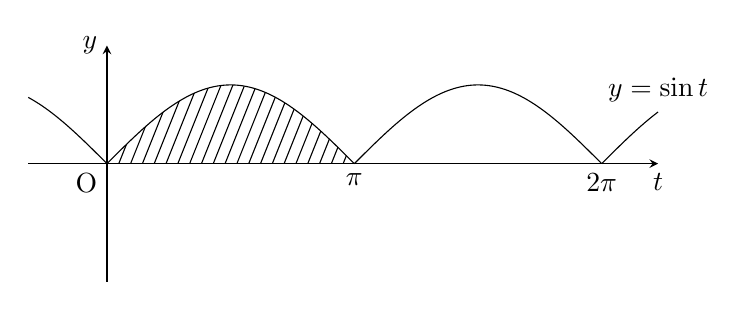
\begin{tikzpicture}
                        \draw [-stealth] (-1,0) -- (7,0) node [below] {$t$};
                        \draw [-stealth] (0,-1.5) -- (0,1.5) node [left] {$y$};
                        \draw [samples=500,domain=-1:0] plot(\x,{-sin(\x r)});
                        \draw [samples=500,domain=0:pi] plot(\x,{sin(\x r)});
                        \draw [samples=500,domain=pi:2*pi] plot(\x,{-sin(\x r)});
                        \draw [samples=500,domain=2*pi:7] plot(\x,{sin(\x r)}) node [above] {$y=\emabs{\sin{t}}$};
                        \draw (0,0) node [below left] {O};
                        \draw (pi,0) node [below] {$\pi$};
                        \draw (2*pi,0) node [below] {$2\pi$};
                        \path[clip] plot [domain=0:pi] (\x,{sin(\x r)}) -- cycle;
                        \foreach \t in {1,2,...,20}{
                            \path[draw] (0.15*\t, 0) -- (0.15*\t+0.4, 1);
                        }
                    \end{tikzpicture}
                    \caption{お山1つ分の面積}
                    \label{お山1つ分の面積}
                }
            \end{figure}

            \textcolor{myBlue2}{したがって,$\dint{k\pi}{(k+1)\pi}\emabs{\sin{t}}\,dt=\dint{0}{\pi}\sin{t}\,dt=\teisekibun{-\cos{t}}{0}{\pi}=-(-1)-(-1)=2$となる.} \\
            $\dint{k\pi}{(k+1)\pi}\emabs{\sin{t}}\,dt=2$であるから,\textcolor{myBlue2}{(この程度の計算の過程は記述をしなくてよいと{\bf 個人的に}思います.)}
            \begin{align*}
                \bunsuu{1}{\sqrt{(k+1)\pi}}\leq A_k \leq \bunsuu{1}{\sqrt{k\pi}}\owari
            \end{align*}
            \item [\kakkoni] \textcolor{myBlue2}{$B_n$は$A_k$と形は似ていますが,少々異なる部分があります.まずは,$B_n$を$A_k$を用いて
            表すことから始めましょう.慣れている人は素早く変形できるかもしれませんが,ここではそのような{\bf プロ}の頭の中を覗いてみましょう.
            文字($B_n$の$n$のこと)で一般化されている場合は,具体的な数字を当てはめることで考えやすくなります.ここで,$B_n$の$\bunsuu{1}{\sqrt{n}}$は邪魔なので,それを除いた
            部分である$\dint{\sqrt{n\pi}}{\sqrt{2n\pi}}\emabs{\sin{(x^2)}}dx$を${B_n}^\prime$と置きます.
            \begin{enumerate}
                \item [\tokeiichi] $n=1$のとき
                \begin{align*}
                    {B_1}^\prime=\dint{\sqrt{\pi}}{\sqrt{2\pi}}\emabs{\sin{(x^2)}}\,dx=A_1
                \end{align*}
                \item [\tokeini] $n=2$のとき
                \begin{align*}
                    {B_2}^\prime&=\dint{\sqrt{2\pi}}{\sqrt{4\pi}}\emabs{\sin{(x^2)}}dx 
                    =\dint{\sqrt{2\pi}}{\sqrt{3\pi}}\emabs{\sin{(x^2)}}\,dx+\dint{\sqrt{3\pi}}{\sqrt{4\pi}}\emabs{\sin{(x^2)}}\,dx 
                    =A_2+A_3
                \end{align*}
                \item [\tokeisan] $n=3$のとき
                \begin{align*}
                    {B_3}^\prime&=\dint{\sqrt{3\pi}}{\sqrt{6\pi}}\emabs{\sin{(x^2)}}dx \\
                    &=\dint{\sqrt{3\pi}}{\sqrt{4\pi}}\emabs{\sin{(x^2)}}\,dx+\dint{\sqrt{4\pi}}{\sqrt{5\pi}}\emabs{\sin{(x^2)}}\,dx+\dint{\sqrt{5\pi}}{\sqrt{6\pi}}\emabs{\sin{(x^2)}}\,dx \\
                    &=A_3+A_4+A_5
                \end{align*}
            \end{enumerate}
            ここまで来れば見えてくるでしょう.
            \begin{align*}
                B_n=\bunsuu{1}{\sqrt{n}}{B_n}^\prime=\bunsuu{1}{\sqrt{n}}\retuwa{k=n}{2n-1}A_k
            \end{align*}
            が得られます.
            } \\
            $B_n=\bunsuu{1}{\sqrt{n}}\retuwa{k=n}{2n-1}A_k$であるから,\kakkoichi で得られた不等式より
            \begin{align*}
                \bunsuu{1}{\sqrt{n}}\retuwa{k=n}{2n-1}\bunsuu{1}{\sqrt{(k+1)\pi}}\leq B_n\leq \bunsuu{1}{\sqrt{n}}\retuwa{k=n}{2n-1}\bunsuu{1}{\sqrt{k\pi}}~\sdots\sdots~\maruni
            \end{align*}
            \textcolor{myBlue2}{この不等式$\maruni$が得られたら,あとは両側の極限をとってはさみうつだけです(簡単なわけではないです).まずは,形がシンプルな
            最右辺の極限を考えてみましょう.} \\
            $\maruni$の最右辺について,区分求積法の原理より
            \begin{align*}
                \dlim{n\to\infty}\bunsuu{1}{\sqrt{n}}\retuwa{k=n}{2n-1}\bunsuu{1}{k\pi}=\dlim{n\to\infty}\bunsuu{1}{n}\retuwa{k=n}{2n-1}\bunsuu{1}{\sqrt{(k/n)\pi}}=\dint{1}{2}\bunsuu{1}{\sqrt{\pi x}}\,dx=\teisekibun{\bunsuu{2\sqrt{x}}{\sqrt{\pi}}}{1}{2}=\bunsuu{2(\sqrt{2}-1)}{\sqrt{\pi}}~\sdots\sdots~\marusan
            \end{align*}
            \textcolor{myBlue2}{と...サクッと計算しましたが,すんなり受け入れられた方は次に進みましょう.計算の過程を詳細に説明します.
            $\lim ,~\retuwa{}{} ,~\bunsuu{1}{n}$の形が見えたら区分求積法を考えましょう.よく見る区分求積法は}
            \begin{mytheo}{定積分と区分求積法}{kubun}
                \textcolor{myBlue2}{$0\leq x\leq 1$において連続な関数$h(x)$において
                \begin{align*}
                    \dlim{n\to\infty}\bunsuu{1}{n}\retuwa{k=1}{n}h\left(\bunsuu{k}{n}\right)=\dint{0}{1}h(x)\,dx
                \end{align*}
                が成り立つ.}
            \end{mytheo}
            \hypersetup{
                linkcolor=myBlue2,
            }
            \textcolor{myBlue2}{ですね.こちらの形に寄せていく($1/n$と$k/n$の形をつくる)と
            \begin{align*}
                \dlim{n\to\infty}\bunsuu{1}{\sqrt{n}}\retuwa{k=n}{2n-1}\bunsuu{1}{k\pi}=\dlim{n\to\infty}\bunsuu{1}{n}\retuwa{k=n}{2n-1}\bunsuu{1}{\sqrt{(k/n)\pi}}
            \end{align*}
            となります.この時点で定理\ref{tha:kubun}における$h(x)$は$h(x)=\bunsuu{1}{\sqrt{\pi x}}$となることが分かります.}
            \hypersetup{
                linkcolor=black,
            }
            \textcolor{myBlue2}{問題なのは$k=n$から$k=2n-1$までの和であるシグマの扱いです.$\dlim{}$の中身を具体的に書き出すと
            \begin{align*}
                \bunsuu{1}{n}\retuwa{k=n}{2n-1}\bunsuu{1}{\sqrt{(k/n)\pi}}=\bunsuu{1}{n}\p{\bunsuu{1}{\sqrt{(n/n)\pi}}+\bunsuu{1}{\sqrt{((n+1)/n)\pi}}+\sdots+\bunsuu{1}{\sqrt{((2n-1)/n)\pi}}}~\sdots\sdots~\marushi
            \end{align*}
            $\marushi$式は以下の網目部の面積を表しています.}
            
            \begin{figure}[htbp]
                \centering
                \textcolor{myBlue2}{
                    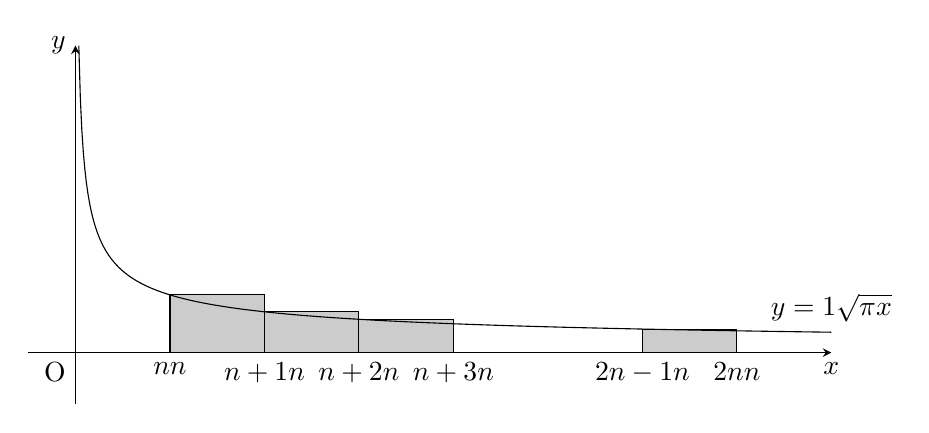
\begin{tikzpicture}[xscale=1.2,yscale=1.3]
                        \draw [-stealth] (-.5,0) -- (8,0) node [below] {$x$};
                        \draw [-stealth] (0,-.5) -- (0,3) node [left] {$y$};
                        \draw [samples=500,domain=0.035368:8] plot(\x,{sqrt(1/(pi*\x))}) node [above] {$y=\bunsuu{1}{\sqrt{\pi x}}$};
                        \draw (0,0) node [below left] {O};
                        \foreach\t in{1,2,3}
                            \draw (\t,0)--(\t,{sqrt(1/(pi*\t))})--(\t+1,{sqrt(1/(pi*\t))})--(\t+1,0);
                        \foreach\t in{1,2,3,6} {
                            \fill [opacity=.2] (\t,0)--(\t,{sqrt(1/(pi*\t))})--(\t+1,{sqrt(1/(pi*\t))})--(\t+1,0);
                            \draw (\t,0)--(\t,{sqrt(1/(pi*\t))})--(\t+1,{sqrt(1/(pi*\t))})--(\t+1,0);
                        }
                        \draw (1,0) node [below] {$\bunsuu{n}{n}$};
                        \draw (2,0) node [below] {$\bunsuu{n+1}{n}$};
                        \draw (3,0) node [below] {$\bunsuu{n+2}{n}$};
                        \draw (4,0) node [below] {$\bunsuu{n+3}{n}$};
                        \draw (6,0) node [below] {$\bunsuu{2n-1}{n}$};
                        \draw (7,0) node [below] {$\bunsuu{2n}{n}$};
                        \draw (5,0) node [below] {\raisebox{-1.2em}{$\sdots\sdots$}};
                        \draw (5,0.1) node {$\sdots\sdots$};
                    \end{tikzpicture}
                    \caption{区分求積法}
                    \label{区分求積法1}
                }
            \end{figure}

            \textcolor{myBlue2}{そして,$1\leq x\leq 2$の範囲で$n$等分された長方形の横の長さ$1/n$を無限に小さくしていく($n\to\infty$とする)と,
            面積は$\dint{1}{2}\bunsuu{1}{\sqrt{\pi x}}$に収束します.(詳細な議論は区分求積法を学んだ教材を復習してください.)したがって
            \begin{align*}
                \dlim{n\to\infty}\bunsuu{1}{n}\retuwa{k=n}{2n-1}\bunsuu{1}{\sqrt{(k/n)\pi}}=\dint{1}{2}\bunsuu{1}{\sqrt{\pi x}}
            \end{align*}
            を得ます.それでは,続いて不等式$\maruni$の最左辺について考えてみましょう.} \\
            $\maruni$の最左辺について,区分求積法の原理より
            \begin{align*}
                \dlim{n\to\infty}\bunsuu{1}{\sqrt{n}}\retuwa{k=n}{2n-1}\bunsuu{1}{\sqrt{(k+1)\pi}}&=\dlim{n\to\infty}\bunsuu{1}{\sqrt{n}}\retuwa{k=n+1}{2n}\bunsuu{1}{\sqrt{k\pi}}=\dlim{n\to\infty}\bunsuu{1}{n}\retuwa{k=n+1}{2n}\bunsuu{1}{\sqrt{(k/n)\pi}} \\
                &=\dint{1}{2}\bunsuu{1}{\sqrt{\pi x}}\,dx=\bunsuu{2(\sqrt{2}-1)}{\sqrt{\pi}}~\sdots\sdots~\marugo
            \end{align*}
            \textcolor{myBlue2}{以下が参考図です.}

            \begin{figure}[htbp]
                \centering
                \textcolor{myBlue2}{
                    \begin{tikzpicture}[xscale=1.2,yscale=1.3]
                        \draw [-stealth] (-.5,0) -- (8,0) node [below] {$x$};
                        \draw [-stealth] (0,-.5) -- (0,3) node [left] {$y$};
                        \draw [samples=500,domain=0.035368:8] plot(\x,{sqrt(1/(pi*\x))}) node [above] {$y=\bunsuu{1}{\sqrt{\pi x}}$};
                        \draw (0,0) node [below left] {O};
                        \foreach\t in{2,3,6,7} {
                            \fill [opacity=.2] (\t-1,0)--(\t-1,{sqrt(1/(pi*\t))})--(\t,{sqrt(1/(pi*\t))})--(\t,0);
                            \draw (\t-1,0)--(\t-1,{sqrt(1/(pi*\t))})--(\t,{sqrt(1/(pi*\t))})--(\t,0);
                        }
                        \draw (1,0) node [below] {$\bunsuu{n}{n}$};
                        \draw (2,0) node [below] {$\bunsuu{n+1}{n}$};
                        \draw (3,0) node [below] {$\bunsuu{n+2}{n}$};
                        \draw (6,0) node [below] {$\bunsuu{2n-1}{n}$};
                        \draw (7,0) node [below] {$\bunsuu{2n}{n}$};
                        \draw (4.5,0) node [below] {\raisebox{-1.2em}{$\sdots\sdots$}};
                        \draw (4,0.1) node {$\sdots\sdots$};
                        \draw (4,2) node [below,align=center] {$(\text{網目部の面積の和})=\bunsuu{1}{n}\retuwa{k=n+1}{2n}\bunsuu{1}{\sqrt{(k/n)\pi}}$}; 
                    \end{tikzpicture}
                    \caption{区分求積法}
                    \label{区分求積法2}
                }
            \end{figure}

            $\maruni,~\marusan,~\marugo$より,はさみうちの原理から$\dlim{n\to\infty}B_n=\boldsymbol{\bunsuu{2(\sqrt{2}-1)}{\sqrt{\pi}}}$となります.\kotae
        \end{enumerate}
\end{document}